\subsubsection{WiFi-Modul}
\label{subsubsec:ESP}

%Aufgrund schon bestehender Erfahrungen wurde für die Wifi-/Bluetooth-Kommunikation ein Espressif ESP-Modul ausgewählt. Grundsätzlich standen zwei Modelle zur Auswahl. Das ESP8266 und das ESP32. Für die Cocktailmaschine wurde das ESP32 ausgewählt, da diese leistungsstärker ist. Die genauen Datenvergleiche sind im Anhang Kapitel \ref{Appendix:ESP32_vs_ESP8266} ersichtlich. Das ESP32 unterstützt das Protokoll nach ISO 802.11 b/g/n und kann somit auf 2.4GHz sowie 5GHz arbeiten. Mit dem n-Protokoll und einer Antenne kann so bis zu 150MBit übertragen werden bei einer Bandbreite von 20MHz.

Das WiFi-/Bluetooth-Modul ist in die Maschine eingebettet, damit der drahtlose Zugriff via Android-Applikation gewährleistet ist. Es handelt sich bei dem Bauteil um das ESP32 vom Hersteller Espressif. Da sich das Bauteil in einer Box befindet, ist es vorteilhaft ein ESP32-Typ zu verwenden, der die Möglichkeit bietet, eine abgesetzte Antenne anzuschliessen, im Falle das Signal zu schwach ist. Dazu eignet sich das Espressif ESP32-32U.

Über den entfernten Zugriff werden folgende Funktionen zur Verfügung gestellt:
\begin{itemize}
\item Applikation per Bluetooth mit dem PartyMixer verbinden.
\item Erstellen von Cocktails.
\item Zuweisung eines Cocktails zu einem Tag.
\item Informationen zur Maschine lesen.
\end{itemize}

%\begin{figure}[!h]
%\center
%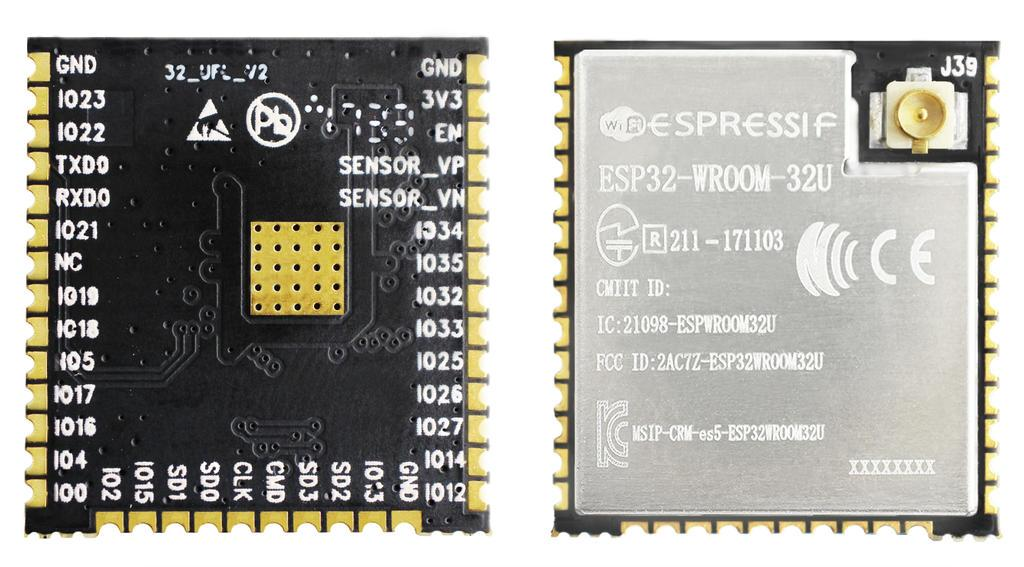
\includegraphics[width = 0.4\textwidth]{graphics/Produktbild_ESP32}
%\caption{ESP32-32U Wroom.}
%\label{fig:Produktbild_ESP32_32U_Wroom}
%\end{figure}
%
%\begin{figure}[!h]
%\center
%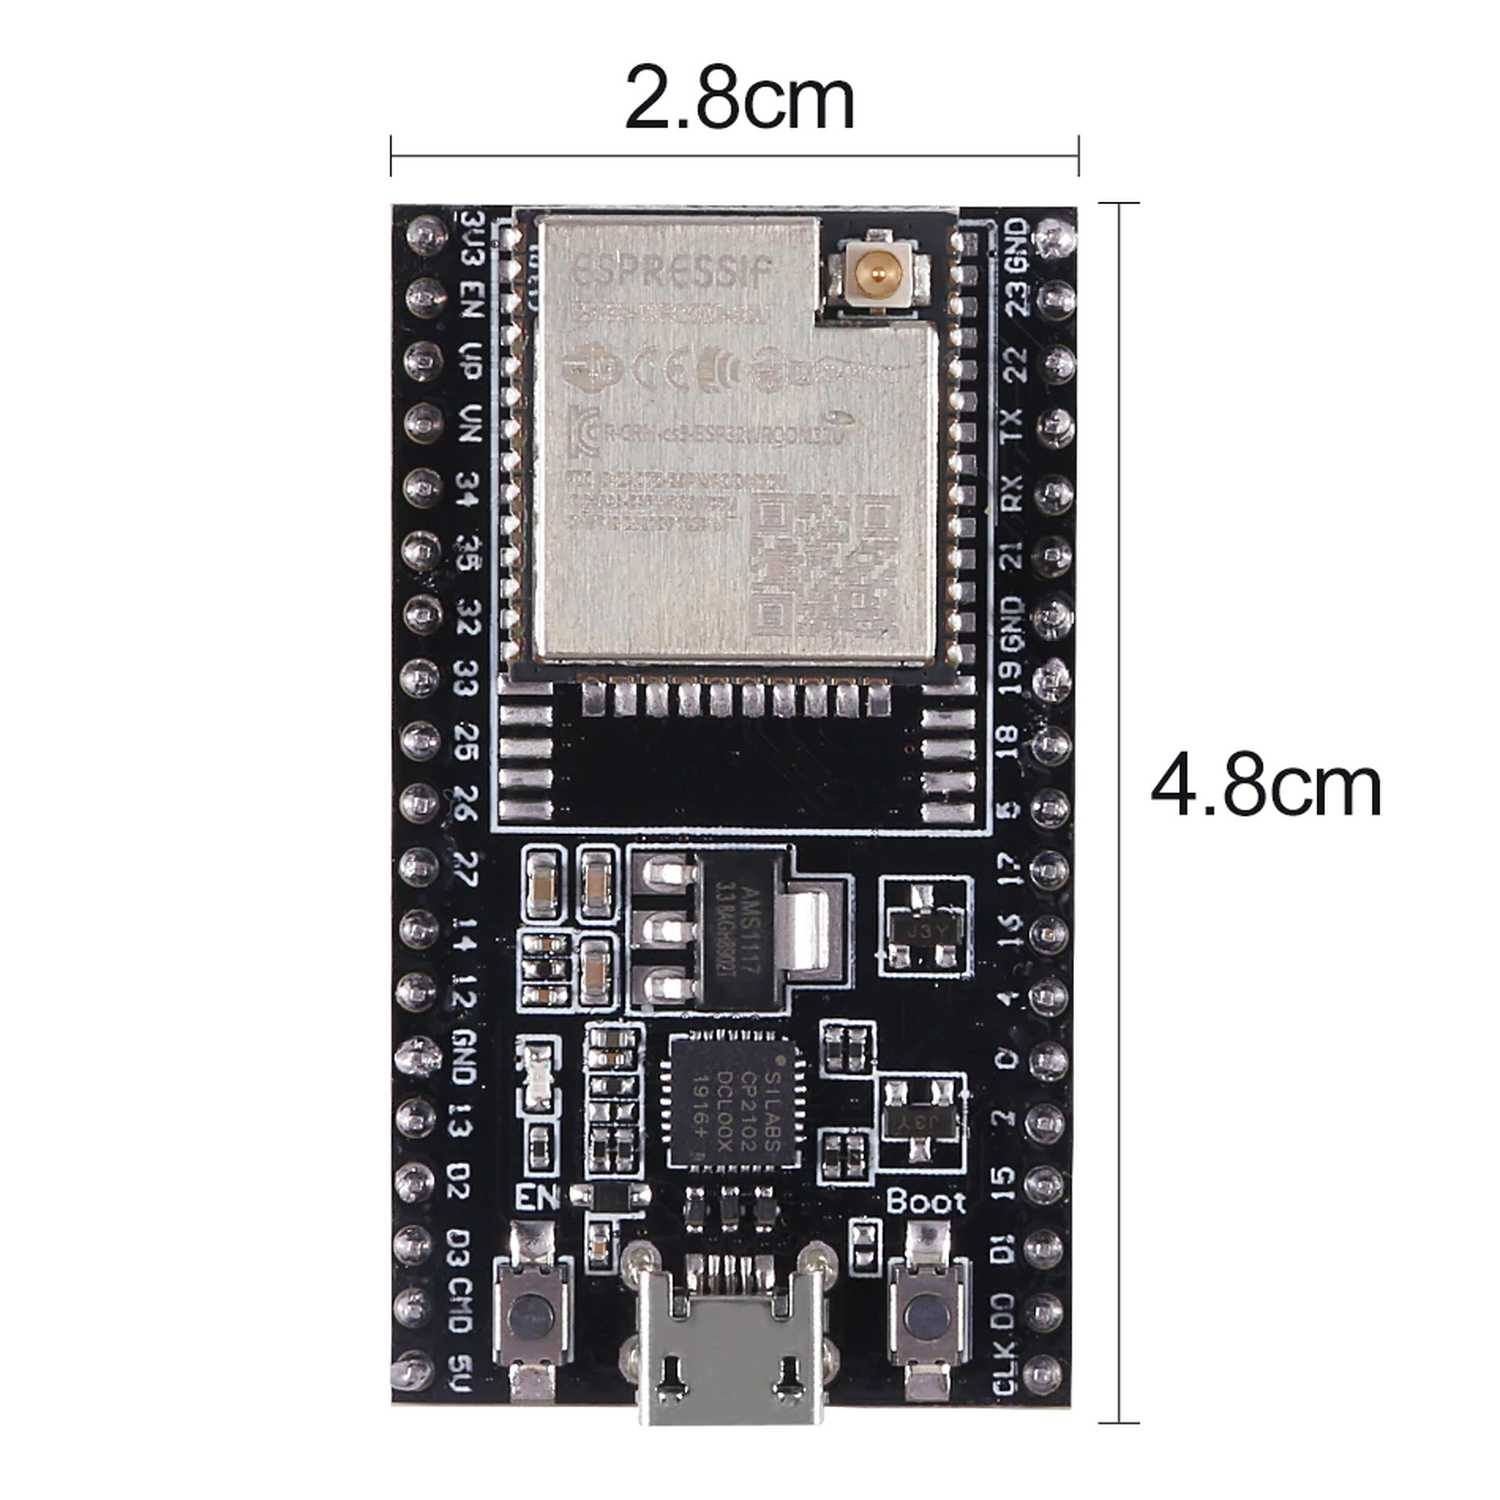
\includegraphics[width = 0.4\textwidth]{graphics/Produktbild_ESP32_2}
%\caption{ESP32-32U DevKit.}
%\label{fig:Produktbild_ESP32_32U_DevKit}
%\end{figure}

\paragraph{Schema (Bluetooth- / Wifimodul)}\mbox{}
\todo{WiFi-Modul? Bluetooth-Modul? WiFi-Bluetooth-Modul??}

Empfängt das WiFi-Modul Daten über Bluetooth, so werden diese Interpretiert und aufbereitet über die zweite serielle Schnittstelle an den Mikrocontroller weitergeleitet. Dieser Vorgang wird mittels Firmware gesteuert. \todo{Evt Referenz auf Beschreibung der App bzw. Software ESP32?}

In Abbildung \ref{fig:Schema_ESP32} ist das Schema des WiFi-Moduls zu sehen. Es beinhaltet Stützkondensatoren, die die Versorgungsspannung glätten sowie die Pull-up- und Pull-down-Widerstände, welche dazu da sind, einen eindeutigen Zustand an den Strapping-Pins zu behalten, während das WiFi-Modul bootet.

In Abbildung \ref{fig:Schema_ESP32_Devkit} ist eine Backup-Lösung zu sehen, wo ein ESP32-Devkit in Header-Pins eingesteckt werden kann. Da die Backup-Lösung nicht gebraucht wird, können die Header-Pins in Abbildung \ref{fig:Schema_ESP32_Devkit} für Korrekturen verwendet werden und dienen so als Backup-Pins für andere Systeme.

\begin{figure}[H]
	\centering
	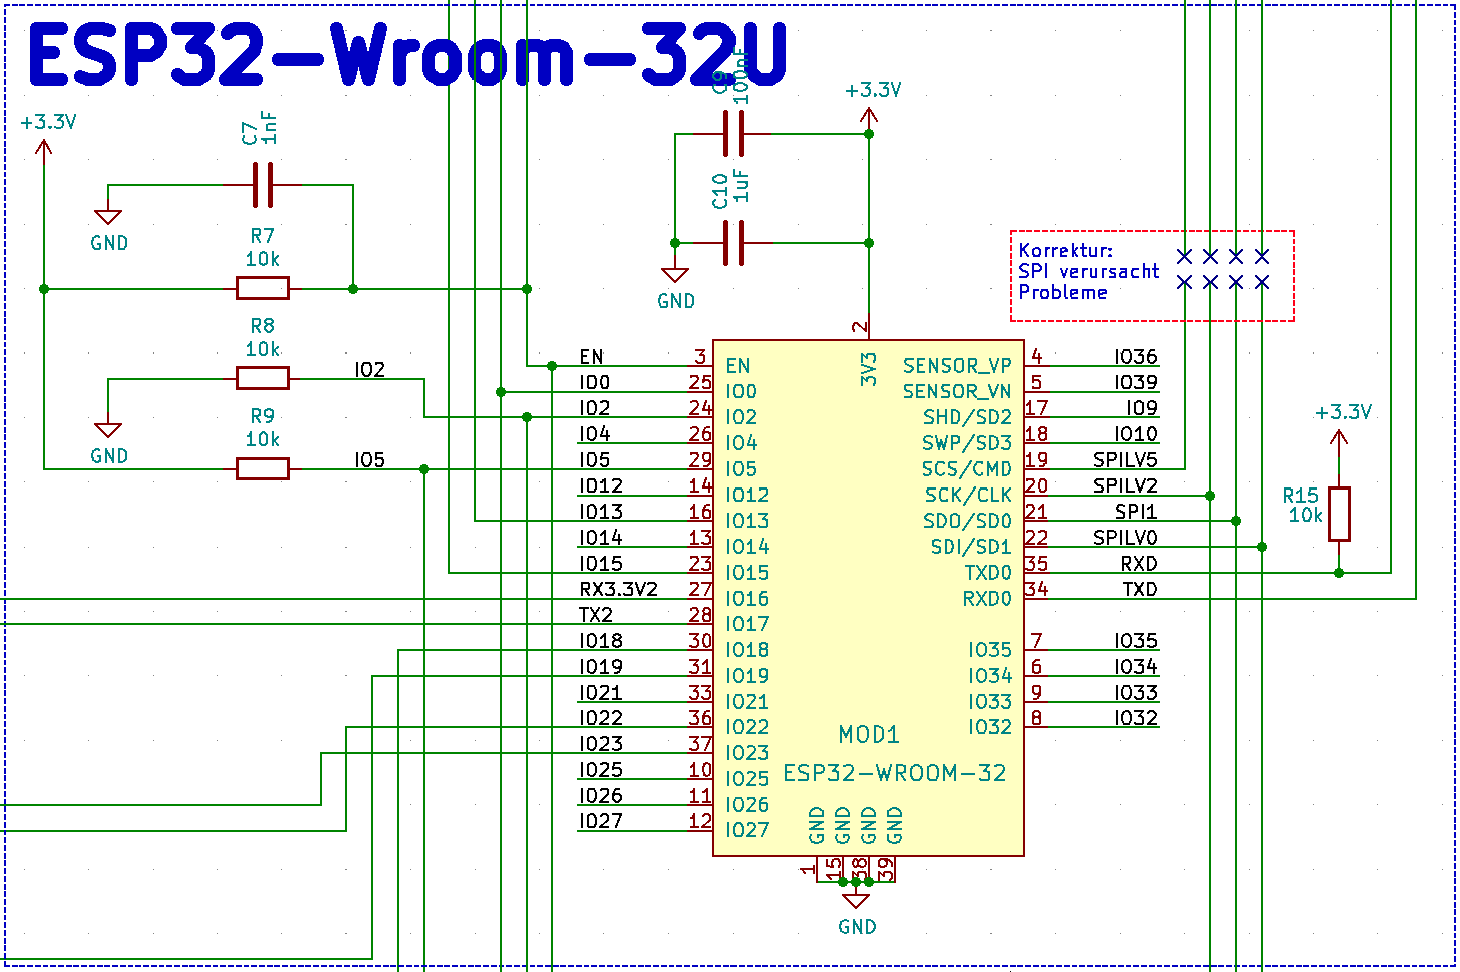
\includegraphics[width=0.8\textwidth]{graphics/Schema_ESP32}
	\caption{Schema ESP32-Wroom-32U.}
	\label{fig:Schema_ESP32}
\end{figure}

\begin{figure}[H]
	\centering
	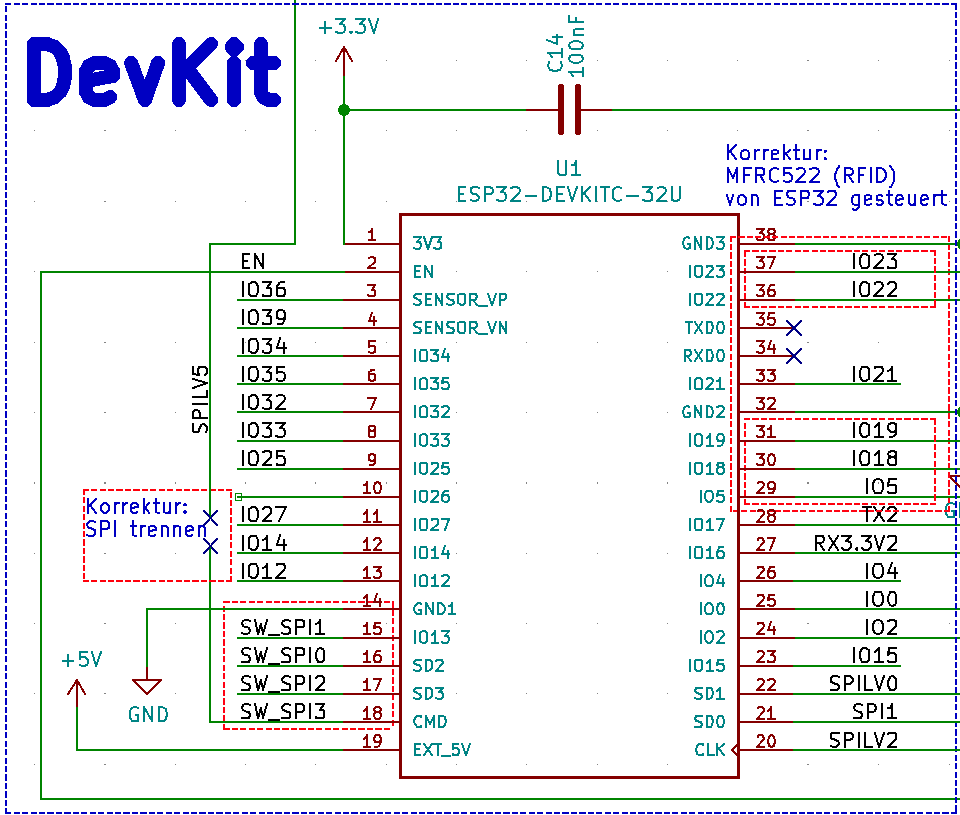
\includegraphics[width=0.5\textwidth]{graphics/Schema_ESP32_Devkit}
	\caption{Header-Pins des DevKits werden für das RFID-Modul und TMC4671 benutzt.}
	\label{fig:Schema_ESP32_Devkit}
\end{figure}

Die Korrekturen an der Hardware wurden Rot eingezeichnet. Die SPI-Verbindung vom Mikrocontroller zum WiFi-Modul, welche in Abbildung \ref{fig:Schema_ESP32} zu sehen ist, ist aufgetrennt, da die Leitungen den Bootvorgang des WiFi-Moduls stören. Aufgrund der funktionierenden Schaltung des ESP32-Wroom und den Störungen, die das RFID-Modul auf dem SPI-Bus verursachte, ist das RFID-Modul am ESP32 über einen separaten SPI-Bus eingesteckt. Deswegen wird die Kommunikation mit dem RFID-Modul vom ESP32 übernommen. Aus dem selben Grund werden die Header-Pins dazu verwendet, eine steckbare Schnittstelle zwischen Mikrocontroller und FOC-Treiber zu bilden. Dazu sind die Leitungen zum ESP32 aufgetrennt und die Pins mit dem Mikrocontroller verbunden.
\newpage
\paragraph{Funktionsbeschrieb der Schaltung (Bluetooth- / Wifimodul)}\mbox{}

Das WiFi-Modul ESP32 ist mit MOD1 beschriftet. Die Kondensatoren C9 und C10 dienen zur Glättung der Eingangsspannung. Über den EN-Pin wird das Modul ein- und ausgeschaltet (acitve high), der Pull-Up-Widerstand R7 zieht diese Leitung defaultmässig auf 5V. Die Widerstände R8, R9, R10 und R11 sind an die Strapping-Pins angeschlossen.
%Über diese werden beim Aufstarten des ESP32 der Boot-Modus, die Versorgungsspannung von VDD\_SDIO\footnote{Secure Digital Input Output}-Slave (Erweiterung der SD-Spezifikationen) und andere Initialisierungseinstellungen konfiguriert.
%Details zu den Konfigurationen sind im Anhang Kapitel \ref{Appendix:ESP32_Strapping} aufgelistet.
Aus Tabelle \ref{tab:Einfluss_Pins_auf_Boot_Modus} ist ersichtlich, dass U0TXD für den normalen Boot-Modus auf HIGH sein muss, weswegen der Widerstand R15 platziert wurde. Mit dem Kondensator C7 wird sichergestellt, dass nach einem Reset automatisch der Download-Boot-Modus gestartet werden kann.

%Wird der Reset-Pin au LOW gezogen, so entlädt sich der Kondensator. Sobald der Reset-Pin auf HIGH gezogen wird, dauert es länger, bis ein logic High-Zustand am CMOS-Eingang erkannt wird. Wird der Pin IO0 auf LOW gezogen, bevor der Enable-Pin nach einem Reset einen HIGH-Zustand erreicht, so wird das ESP32 in den Download-Boot-Modus gesetzt. Das Setzen

\paragraph{Schema (Automatische Boot-Logik)}\mbox{}

Die automatischen Bootlogik, welche in Abbildung \ref{fig:Schema_ESP32_Flashbuttons} zu sehein ist, steuert die Pins EN und IO0 so an, dass das WiFi-Modul beim Hochladen eines Programms automatisch neu gestartet wird und die Spannung an den Pins so anliegt, dass der Download-Boot-Modus gestartet wird.

\begin{figure}[H]
	\centering
	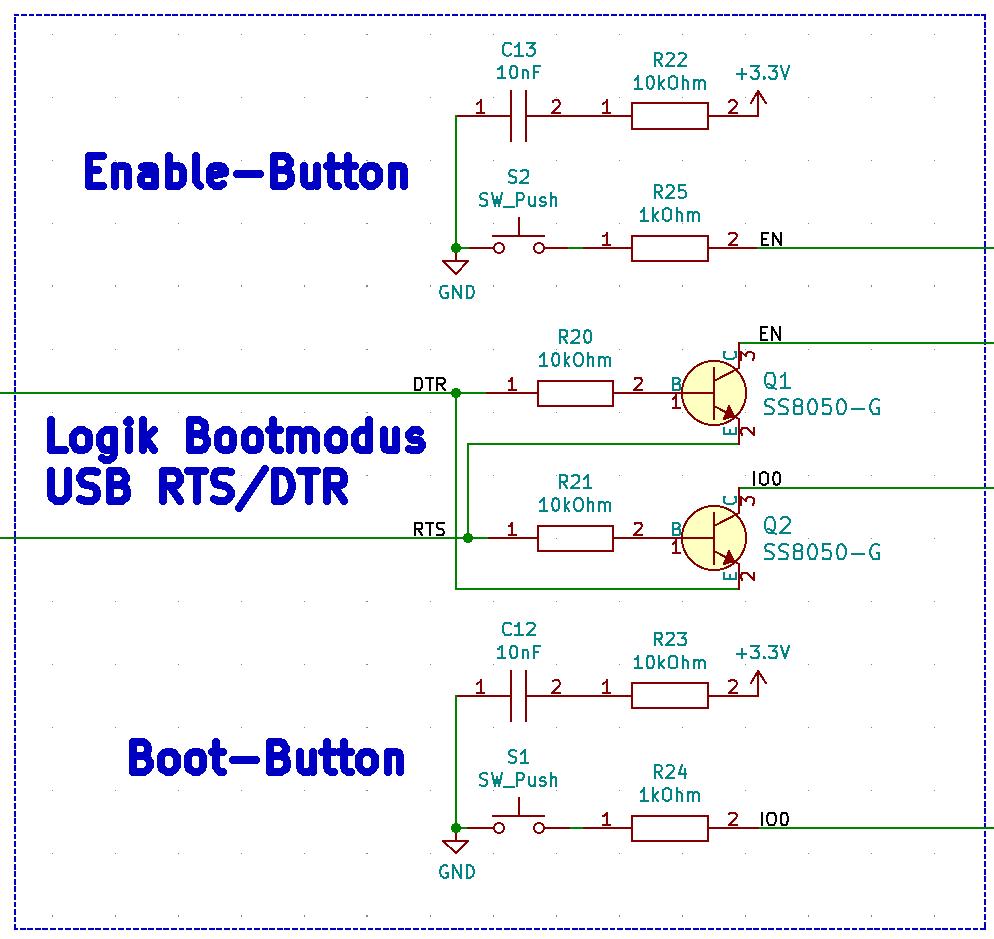
\includegraphics[width=0.7\textwidth]{graphics/Schema_ESP32_Flashbuttons}
	\caption{Schema automatische Bootlogik.}
	\label{fig:Schema_ESP32_Flashbuttons}
\end{figure}

\paragraph{Funtionsbeschrieb der Schaltung (Automatische Bootlogik)}\mbox{}

Für die Beschaltung der automatischen Boot-Logik benötigt es die Leitungen DTR und RTS, welche vom USB-UART-Konverter gesteuert werden und EN und IO0 als Outputs auf das WiFi-Modul. Die Buttons sind dazu da, das ESP manuell in den Download-Boot-Modus zu setzen.
Die Widerstände R20 und R21 sind Vorwiderstände an der Basis der Transistoren Q1 und Q2. R22 und R23 sind Pull-Up-Widerstände für die EN- und IO0-Leitung. Die Kondensatoren C13 und C12 dienen dem Entprellen der Buttons. Die Widerstände R25 und R24 begrenzen den Strom bei Drücken der Buttons S1 oder S2.
